\documentclass[11pt]{article}
\usepackage{fullpage,url}
\usepackage{amsmath,amsthm,amssymb}
\usepackage{graphicx}
\usepackage{eso-pic}
\usepackage{bm}
\usepackage{caption}
\usepackage{picins}   
\usepackage{microtype}
\usepackage{multirow}
\usepackage{url}
\usepackage{enumerate}
%\usepackage{tabular}

\usepackage[letterpaper,top=1in,bottom=1in,left=1in,right=1in,nohead]{geometry}

\newenvironment{claim}[1]{\noindent\underline{{\bf Claim:}}\space#1}{}
\newenvironment{claimproof}[1]{\par\noindent\underline{{\bf Proof:}}\space#1}
{\hfill$\square$}

\makeatletter
\newcommand{\specialnumber}[1]{%
  \def\tagform@##1{\maketag@@@{(\ignorespaces##1\unskip\@@italiccorr#1)}}%
}

\setlength{\parindent}{0in}
\setlength{\parskip}{6pt}

\DeclareMathOperator{\E}{E}
\DeclareMathOperator{\Var}{Var}
\DeclareMathOperator{\Unif}{Unif}

\begin{document}
\thispagestyle{empty}
{\large{\bf CS6957: Probabilistic Modeling \hfill Prateep Mukherjee(u0876583)}}\\

{\LARGE{\bf Homework 2}}
\vspace{0.2\baselineskip}
\hrule

\section{}  
\label{1}

The total number of probabilities needed to store the network is product of the number of values for all the variables. Therefore, the result is $ [8(income) * 2(exercise) * 2(smoke) * 4(bmi) * 4(bp) * 2(cholesterol)  * 2(angina) * 2(stroke) * 2(attack)  * 4(diabetes) ] = 32768$.

%\par
%\large{
%For this homework, I discussed the procedure of \textbf{marginalize} with \textbf{Sayan Dey. }
%}
\vspace{-10pt}

\section{(a)} 
\label{r2}
%% Diabetes | habits
p(Diabetes $|$ bad habits)

\begin{table*}[!hbt]
\begin{center}
\begin{tabular}{ |c|c|c|c| }
  \hline
  probs & smoke & exercise & diabetes \\
  \hline
  0.136660053 & 1 & 2 & 1 \\
  \hline
  0.008914666 & 1 & 2 & 2 \\
  \hline
  0.837385140  & 1  &     2 &    3 \\
  \hline
  0.017040141  &    1    & 2   & 4 \\
  \hline
\end{tabular}
\end{center}
\end{table*}
\vspace{-20pt}
 
p(Diabetes $|$ good habits)

\begin{table*}[!hbt]
\begin{center}
\begin{tabular}{ |c|c|c|c| }
  \hline
  probs & smoke & exercise & diabetes \\
  \hline
  0.131893738 & 2 & 1 & 1 \\
  \hline
  0.008881042 & 2 & 1 & 2 \\
  \hline
  0.842538131  & 2  &     1 &    3 \\
  \hline
  0.016687089  &    2    & 1   & 4 \\
  \hline
\end{tabular}
\end{center}
\end{table*}
\vspace{-20pt}

%% Stroke | habits
p(Stroke $|$ bad habits)

\begin{table*}[!hbt]
\begin{center}
\begin{tabular}{ |c|c|c|c| }
  \hline
  probs & smoke & exercise & stroke \\
  \hline
  0.04959854 & 1 & 2 & 1 \\
  \hline
  0.95040146 & 1 & 2 & 2 \\
  \hline
\end{tabular}
\end{center}
\end{table*}
\vspace{-20pt}

p(Stroke $|$ good habits)

\begin{table*}[!hbt]
\begin{center}
\begin{tabular}{ |c|c|c|c| }
  \hline
  probs & smoke & exercise & stroke \\
  \hline
  0.03605402 & 2 & 1 & 1 \\
  \hline
  0.96394598 & 2 & 1 & 2 \\
  \hline
\end{tabular}
\end{center}
\end{table*}
\vspace{-20pt}

%% Attack | habits
p(Attack $|$ bad habits)

\begin{table*}[!hbt]
\begin{center}
\begin{tabular}{ |c|c|c|c| }
  \hline
  probs & smoke & exercise & attack \\
  \hline
  0.0742565 & 1 & 2 & 1 \\
  \hline
  0.9257435 & 1 & 2 & 2 \\
  \hline
\end{tabular}
\end{center}
\end{table*}
\vspace{-20pt}

\clearpage

p(Attack $|$ good habits)

\begin{table*}[!hbt]
\begin{center}
\begin{tabular}{ |c|c|c|c| }
  \hline
  probs & smoke & exercise & attack \\
  \hline
  0.05287024 & 2 & 1 & 1 \\
  \hline
 0.94712976 & 2 & 1 & 2 \\
  \hline
\end{tabular}
\end{center}
\end{table*}
\vspace{-20pt}

%% Angina | habits
p(Angina $|$ bad habits)

\begin{table*}[!hbt]
\begin{center}
\begin{tabular}{ |c|c|c|c| }
  \hline
  probs & smoke & exercise & angina \\
  \hline
 0.08008408 & 1 & 2 & 1 \\
  \hline
 0.91991592 & 1 & 2 & 2 \\
  \hline
\end{tabular}
\end{center}
\end{table*}
\vspace{-20pt}

p(Angina $|$ good habits)

\begin{table*}[!hbt]
\begin{center}
\begin{tabular}{ |c|c|c|c| }
  \hline
  probs & smoke & exercise & angina \\
  \hline
 0.05488682 & 2 & 1 & 1 \\
  \hline
 0.94511318 & 2 & 1 & 2 \\
  \hline
\end{tabular}
\end{center}
\end{table*}

\vspace{-20pt}

\par \textbf{(b)}
% Diabetes | health

p(Diabetes $|$ poor health)

\begin{table*}[!hbt]
\begin{center}
\begin{tabular}{ |c|c|c|c|c| }
  \hline
  probs & diabetes & bmi & cholesterol & bp \\
  \hline
  0.115422719 & 1 & 3 & 1 & 1\\
  \hline
  0.007661825 & 2 & 3 & 1 & 1 \\
  \hline
  0.860872761  & 3  &  3 &  1 & 1 \\
  \hline
  0.016042695  &   4    & 3   & 1 & 1 \\
  \hline
\end{tabular}
\end{center}
\end{table*}
\vspace{-20pt}

p(Diabetes $|$ good health)

\begin{table*}[!hbt]
\begin{center}
\begin{tabular}{ |c|c|c|c|c| }
  \hline
  probs & diabetes & bmi & cholesterol & bp \\
  \hline
  0.057709954 & 1 & 2 & 2 & 3\\
  \hline
  0.009543386 & 2 & 2 & 2 & 3 \\
  \hline
  0.922193878  & 3  &  2 &  2 & 3 \\
  \hline
  0.010552782  &   4  & 2   & 2 & 3 \\
  \hline
\end{tabular}
\end{center}
\end{table*}
\vspace{-20pt}

% Stroke | health

p(Stroke $|$ poor health)

\begin{table*}[!hbt]
\begin{center}
\begin{tabular}{ |c|c|c|c|c| }
  \hline
  probs & stroke & bmi & bp & cholesterol \\
  \hline
  0.08268577 & 1 & 3 & 1 & 1\\
  \hline
  0.91731423 & 2 & 3 & 1 & 1 \\
  \hline
\end{tabular}
\end{center}
\end{table*}
\vspace{-20pt}

p(Stroke $|$ good health)

\begin{table*}[!hbt]
\begin{center}
\begin{tabular}{ |c|c|c|c|c| }
  \hline
  probs & stroke & bmi & bp & cholesterol \\
  \hline
  0.01446014 & 1 & 2 & 3 & 2\\
  \hline
  0.98553986 & 2 & 2 & 3 & 2 \\
  \hline
\end{tabular}
\end{center}
\end{table*}
\vspace{-20pt}

\clearpage

% Attack | health

p(Attack $|$ poor health)

\begin{table*}[!hbt]
\begin{center}
\begin{tabular}{ |c|c|c|c|c| }
  \hline
  probs & attack & bmi & bp & cholesterol \\
  \hline
  0.1407844 & 1 & 3 & 1 & 1\\
  \hline
  0.8592156 & 2 & 3 & 1 & 1 \\
  \hline
\end{tabular}
\end{center}
\end{table*}
\vspace{-20pt}

p(Attack $|$ good health)

\begin{table*}[!hbt]
\begin{center}
\begin{tabular}{ |c|c|c|c|c| }
  \hline
  probs & attack & bmi & bp & cholesterol \\
  \hline
  0.01616133 & 1 & 2 & 3 & 2\\
  \hline
  0.98383867 & 2 & 2 & 3 & 2 \\
  \hline
\end{tabular}
\end{center}
\end{table*}
\vspace{-20pt}

% Angina | health

p(Angina $|$ poor health)

\begin{table*}[!hbt]
\begin{center}
\begin{tabular}{ |c|c|c|c|c| }
  \hline
  probs & angina & bmi & bp & cholesterol \\
  \hline
  0.1616076 & 1 & 3 & 1 & 1\\
  \hline
  0.8383924 & 2 & 3 & 1 & 1 \\
  \hline
\end{tabular}
\end{center}
\end{table*}
\vspace{-20pt}

p(Angina $|$ good health)

\begin{table*}[!hbt]
\begin{center}
\begin{tabular}{ |c|c|c|c|c| }
  \hline
  probs & angina & bmi & bp & cholesterol \\
  \hline
  0.01332601 & 1 & 2 & 3 & 2\\
  \hline
  0.98667399 & 2 & 2 & 3 & 2 \\
  \hline
\end{tabular}
\end{center}
\end{table*}
\vspace{-20pt}

\section{}
\label{3}
\vspace{-20pt}
  From Fig. \ref{fig3}, the inference is that as a person's annual income level goes higher, the probability of all the health outcomes reduces.
%\vspace{-20pt}
\begin{figure*}[!h]
\begin{center}
  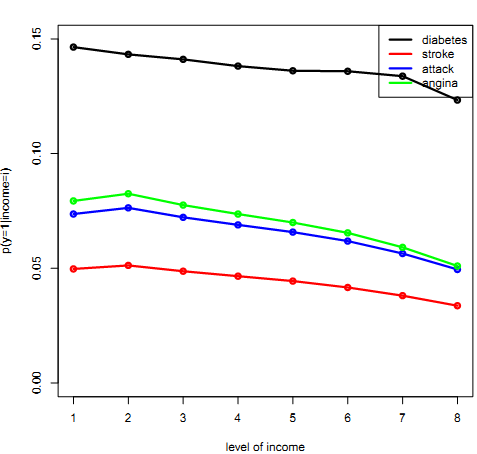
\includegraphics[scale=0.6]{3_plots}
\end{center}
\vspace{-20pt}
\caption{\small{Probability of health outcome(diabetes, stroke, heart attack, angina) for each level of annual income. Annual income is plotted in 8 different levels.  Posterior  probability $P(y=1|income=i)$ is normalized to [0,0.15]. }}
\label{fig3}
\end{figure*}

\section{} 
\label{4}

As there are no links between the habits(smoking and exercise) and the outcomes, the assumption is that there are no direct effects of smoking and exercise on the diseases. Next, we add links between the habits and the outcomes. The following tables show the inference measures obtained.

%\clearpage

% Diabetes | habits

p(Diabetes $|$ bad habits)

\begin{table*}[!hbt]
\begin{center}
\begin{tabular}{ |c|c|c|c| }
  \hline
  probs & smoke & exercise & diabetes \\
  \hline
  0.210944859 & 1 & 2 & 1 \\
  \hline
  0.006915095 & 1 & 2 & 2 \\
  \hline
  0.760692694  & 1  &     2 &    3 \\
  \hline
  0.021447352  &    1    & 2   & 4 \\
  \hline
\end{tabular}
\end{center}
\end{table*}
\vspace{-20pt}
 
p(Diabetes $|$ good habits)

\begin{table*}[!hbt]
\begin{center}
\begin{tabular}{ |c|c|c|c| }
  \hline
  probs & smoke & exercise & diabetes \\
  \hline
  0.098552162 & 2 & 1 & 1 \\
  \hline
  0.009884084 & 2 & 1 & 2 \\
  \hline
  0.877575578  & 2  &     1 &    3 \\
  \hline
  0.013988176  &    2    & 1   & 4 \\
  \hline
\end{tabular}
\end{center}
\end{table*}
\vspace{-20pt}

% Diabetes | health

p(Diabetes $|$ poor health)

\begin{table*}[!hbt]
\begin{center}
\begin{tabular}{ |c|c|c|c|c| }
  \hline
  probs & diabetes & bmi & cholesterol & bp \\
  \hline
  0.123480634 & 1 & 3 & 1 & 1\\
  \hline 
  0.007460298 & 2 & 3 & 1 & 1 \\
  \hline
  0.852415963  & 3  &  3 &  1 & 1 \\
  \hline
  0.016643105  &   4    & 3   & 1 & 1 \\
  \hline
\end{tabular}
\end{center}
\end{table*}
\vspace{-20pt}

p(Diabetes $|$ good health)

\begin{table*}[!hbt]
\begin{center}
\begin{tabular}{ |c|c|c|c|c| }
  \hline
  probs & diabetes & bmi & cholesterol & bp \\
  \hline
  0.054172949 & 1 & 2 & 2 & 3\\
  \hline
  0.009731215 & 2 & 2 & 2 & 3 \\
  \hline
  0.925952333  & 3  &  2 &  2 & 3 \\
  \hline
  0.010143502  &   4  & 2   & 2 & 3 \\
  \hline
\end{tabular}
\end{center}
\end{table*}
\vspace{-20pt}

%% Stroke | habits
p(Stroke $|$ bad habits)

\begin{table*}[!hbt]
\begin{center}
\begin{tabular}{ |c|c|c|c| }
  \hline
  probs & smoke & exercise & stroke \\
  \hline
  0.07803498 & 1 & 2 & 1 \\
  \hline
  0.92196502 & 1 & 2 & 2 \\
  \hline
\end{tabular}
\end{center}
\end{table*}
\vspace{-20pt}

p(Stroke $|$ good habits)

\begin{table*}[!hbt]
\begin{center}
\begin{tabular}{ |c|c|c|c| }
  \hline
  probs & smoke & exercise & stroke \\
  \hline
  0.02431088 & 2 & 1 & 1 \\
  \hline
  0.97568912 & 2 & 1 & 2 \\
  \hline
\end{tabular}
\end{center}
\end{table*}
\vspace{-20pt}

\clearpage

% Stroke | health

p(Stroke $|$ poor health)

\begin{table*}[!hbt]
\begin{center}
\begin{tabular}{ |c|c|c|c|c| }
  \hline
  probs & stroke & bmi & bp & cholesterol \\
  \hline
  0.08425692 & 1 & 3 & 1 & 1\\
  \hline
  0.91574308 & 2 & 3 & 1 & 1 \\
  \hline
\end{tabular}
\end{center}
\end{table*}

p(Stroke $|$ good health)

\begin{table*}[!hbt]
\begin{center}
\begin{tabular}{ |c|c|c|c|c| }
  \hline
  probs & stroke & bmi & bp & cholesterol \\
  \hline
  0.01399739 & 1 & 2 & 3 & 2\\
  \hline
 0.98600261 & 2 & 2 & 3 & 2 \\
  \hline
\end{tabular}
\end{center}
\end{table*}
\vspace{-20pt}

%% Attack | habits
p(Attack $|$ bad habits)

\begin{table*}[!hbt]
\begin{center}
\begin{tabular}{ |c|c|c|c| }
  \hline
  probs & smoke & exercise & attack \\
  \hline
  0.1211659 & 1 & 2 & 1 \\
  \hline
  0.8788341 & 1 & 2 & 2 \\
  \hline
\end{tabular}
\end{center}
\end{table*}
\vspace{-20pt}

p(Attack $|$ good habits)

\begin{table*}[!hbt]
\begin{center}
\begin{tabular}{ |c|c|c|c| }
  \hline
  probs & smoke & exercise & attack \\
  \hline
  0.03101531 & 2 & 1 & 1 \\
  \hline
 0.96898469 & 2 & 1 & 2 \\
  \hline
\end{tabular}
\end{center}
\end{table*}
\vspace{-20pt}

% Attack | health

p(Attack $|$ poor health)

\begin{table*}[!hbt]
\begin{center}
\begin{tabular}{ |c|c|c|c|c| }
  \hline
  probs & attack & bmi & bp & cholesterol \\
  \hline
  0.1421993 & 1 & 3 & 1 & 1\\
  \hline
  0.8578007 & 2 & 3 & 1 & 1 \\
  \hline
\end{tabular}
\end{center}
\end{table*}
\vspace{-20pt}


p(Attack $|$ good health)

\begin{table*}[!hbt]
\begin{center}
\begin{tabular}{ |c|c|c|c|c| }
  \hline
  probs & attack & bmi & bp & cholesterol \\
  \hline
  0.01546893 & 1 & 2 & 3 & 2\\
  \hline
  0.98453107 & 2 & 2 & 3 & 2 \\
  \hline
\end{tabular}
\end{center}
\end{table*}
\vspace{-20pt}

%% Angina | habits
p(Angina $|$ bad habits)

\begin{table*}[!hbt]
\begin{center}
\begin{tabular}{ |c|c|c|c| }
  \hline
  probs & smoke & exercise & angina \\
  \hline
 0.1190069 & 1 & 2 & 1 \\
  \hline
 0.8809931  & 1 & 2 & 2 \\
  \hline
\end{tabular}
\end{center}
\end{table*}
\vspace{-20pt}

p(Angina $|$ good habits)

\begin{table*}[!hbt]
\begin{center}
\begin{tabular}{ |c|c|c|c| }
  \hline
  probs & smoke & exercise & angina \\
  \hline
 0.03680005 & 2 & 1 & 1 \\
  \hline
 0.96319995 & 2 & 1 & 2 \\
  \hline
\end{tabular}
\end{center}
\end{table*}
\vspace{-20pt}

\clearpage

% Angina | health

p(Angina $|$ poor health)

\begin{table*}[!hbt]
\begin{center}
\begin{tabular}{ |c|c|c|c|c| }
  \hline
  probs & angina & bmi & bp & cholesterol \\
  \hline
  0.1629716 & 1 & 3 & 1 & 1\\
  \hline
  0.8370284 & 2 & 3 & 1 & 1 \\
  \hline
\end{tabular}
\end{center}
\end{table*}
\vspace{-20pt}

p(Angina $|$ good health)

\begin{table*}[!hbt]
\begin{center}
\begin{tabular}{ |c|c|c|c|c| }
  \hline
  probs & angina & bmi & bp & cholesterol \\
  \hline
  0.01294426 & 1 & 2 & 3 & 2\\
  \hline
  0.98705574 & 2 & 2 & 3 & 2 \\
  \hline
\end{tabular}
\end{center}
\end{table*}

\par The above tables show that probability for people having good habits and health for not having any health outcomes increase. Similarly, probability for people having health outcomes given they have poor habits and health increases. This shows that our assumption in question \ref{2} is not valid.

\section{}
\label{5}

The bayesian net in question \label{2} assumes no direct link between the health outcomes. After we introduce such links, the probability that a person can get stroke given he already has diabetes increases. Similarly, probability that he can get stroke given that he does not have diabetes decreases. 

\begin{table*}[!hbt]
\begin{center}
\begin{tabular}{ |c|c| }
  \hline
  %probs & angina & bmi & bp & cholesterol \\
  $P_{old}$(stroke = 1 $|$ diabetes=1) & $P_{new}$(stroke=1 $|$ diabetes=1) \\
  \hline
  0.04416376 & 0.07619782 \\
  \hline
\end{tabular}
\end{center}
\end{table*}

\begin{table*}[!hbt]
\begin{center}
\begin{tabular}{ |c|c| }
  \hline
  %probs & angina & bmi & bp & cholesterol \\
  $P_{old}$(stroke = 1 $|$ diabetes=3) & $P_{new}$(stroke=1 $|$ diabetes=3) \\
  \hline
  0.04047831 & 0.03501533 \\
  \hline
\end{tabular}
\end{center}
\end{table*}

The above tables show that the above assumption is not valid.


\end{document}